\chapter{METHODOLOGY}\label{METHODOLOGY}

This chapter discusses about the methodology that has been used to carry out the thesis work. The research is carried out using two approaches: Classical Machine Learning approach and Federated Learning approach.

\section{Identification of Research Gaps} 
Defining the system's goals and reading certain literature reviews are the first steps of the applied research methodology. The primary goals of the thesis are presented and the dataset of pap smear test cervical cell images is acquired. Then two approaches were followed for classification of those images.  

\section{Classical ML approach}
In this first approach, fifteen different Machine Learning models have been applied to train the model to determine which would provide an overall increased accuracy. Subsequently, the models are compared with respect to the accuracy, precision, recall and f1-score of the training set and the accuracy, precision and recall of the test set.

\section{Federated Learning Approach}
In the second approach, various CNN models were developed and integrated with FL architecture. Hyperparameter tuning was done to figure out the best possible architecture. After evaluating the models, the best model was deployed through streamlit and a user interface was designed in order to apply the proposed system in a real-world environment. 

\begin{figure}[H]
\centering
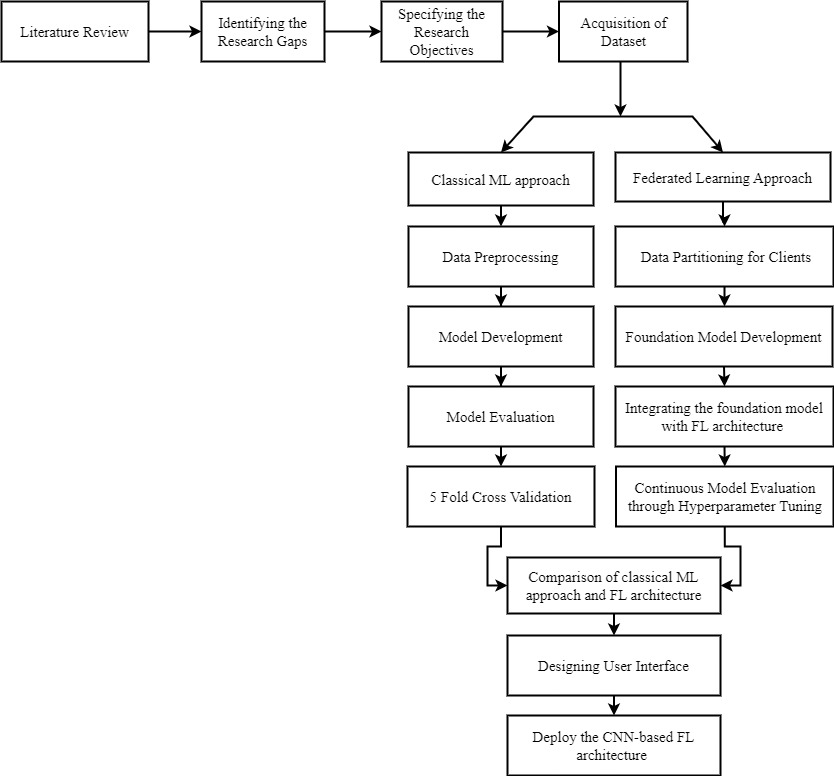
\includegraphics[width=148mm,height=140mm]{figures/meth.jpg}
\caption{Overview of Methodology}
\label{DLAccuracy}
\end{figure}

An overview of methodology is shown in Fig 4.1. By following this methodology, a conclusion was reached that FL performs significantly better than classical ML models.


\endinput

